% Lecture for ph2a Caltech 2017: Vibrations and Waves
\documentclass[pdf, handout, hideothersubsections]{beamer}
\usepackage{beamerthemeshadow}
\mode<presentation>
  {
    \usefonttheme{structuresmallcapsserif}
    \usetheme{CambridgeUS}
    \usecolortheme{seahorse}
    %\useinnertheme{circles}
%    \useoutertheme{tree}
  }

\usepackage{svg}
\usepackage{xmpmulti}
\usepackage{bm}
\usepackage{mathtools}
%\usepackage{enumitem}
\usepackage{hyperref}
\hypersetup{
    pdffitwindow=true,     % window fit to page when opened
    colorlinks=true,       % false: boxed links; true: colored links
    linkcolor=orange,      % color of internal links 
    citecolor=green,       % color of links to bibliography
    filecolor=magenta,     % color of file links
    urlcolor=blue,         % color of external links
    pdfstartview={Fit}
}

% Fonts/encoding
\renewcommand{\UrlFont}{\tiny}
\usepackage[utf8]{inputenc}
\usepackage[T1]{fontenc}
%\usepackage[sc,medium,raggedright]{titlesec}
\usepackage{newtxmath}
%\usepackage{libertine}
\usepackage[osf]{ebgaramond}

\graphicspath{{Figures/}}

\begin{document}
\title{Fourier Analysis}  
\author{Caltech: ph2a}
\date{19 - Oct - 2017}


\frame{\titlepage} 

\frame{\frametitle{Table of Contents}\tableofcontents} 

\setbeamerfont{footnote}{size=\tiny}

\section{Summary}
\begin{frame}
\frametitle{Last Time:}
\begin{enumerate}
  \pause
\item Matrix methods can be used to analyzed eigenmodes of linear systems.
  \pause
\item The case of $N$ springs and $N$ masses can be analyzed as a
  straightforward extension of the methods used for $N = 2, 3$.
  \pause
\item Strings are an extension of this method to $N \rightarrow \infty$.
  \pause
\item The Bode plot for systems with finite $N$, and then 
  infinite $N$, illustrates the phenomena of \emph{dispersion} and the
  \emph{cut-off} frequency.
\pause
\item The rest of this course is the study of waves. This week we make
  the gradual transition between vibrations of discrete elements to
  waves: vibrations in continuous systems.
\end{enumerate}
\end{frame}


\begin{frame}
\frametitle{Overview}
\pause
\begin{itemize}
\item Fourier Analysis: decompose solutions into sinusoidal components
  of different frequencies
  (French pp. 189\,--\,196)
  \pause
\item $y(x, t) \rightarrow \tilde{y}(f, t)$
  \pause
\item The \emph{Fourier Transform} converts a function from the
  time-domain into the frequency-domain.
  \pause
\item The inverse Fourier Transform does the inverse and returns to us
  the time domain signal.
  \pause
\item Functions which are made up primarily of sinusoids are
  efficiently described in the frequency domain (e.g. harmonic
  oscillators) using tools like the Bode Plot and Power Spectrum.
  \pause
\item We know the SHO solutions are just sinusoids, so \emph{any}
  arbitrary shape, $y(x,t)$, can be decomposed into these Fourier
  components and then evolved in time.
\pause
\item Fourier analysis is a specific case of the general method of
  Hilbert space analysis where the basis functions can be anything,
  not just sine waves. (e.g. Laplace is for SHO + damping)
\end{itemize}
\end{frame}


\section{Fourier Analysis of Waves}

\begin{frame}
  \frametitle{Fourier Analysis of String}
  \pause
  \begin{itemize}
  \item General Solution: $y(x, t) = \sum_{n=1}^{\infty} A_n cos(\omega_n t - \phi_0) sin(\frac{n \pi x}{L})$
    \pause
  \item Step \#1: Applying boundary conditions -
    \pause
  \item $y(x, 0) = \sum_{n=1}^{\infty} A_n cos(\phi_0) sin(\frac{n \pi x}{L})$
    \pause
  \item $\dot{y}(x, 0) = \sum_{n=1}^{\infty} A_n \omega_n sin(\phi_0)
    sin(\frac{n \pi x}{L})$
    \pause
  \item Since $A_n$ and $\phi_0$ are constants (not dependent on
    time), we now have $y(x, t)$; just need to find $A_n$ and $\phi_0$.
    \pause
  \item For compactness of notation, let $B_n \equiv A_n cos(\phi_0)$
    and $C_n \equiv A_n sin(\phi_0)$.
  \end{itemize}

\end{frame}

\begin{frame}
\frametitle{Waves of Different Frequencies are like unit vectors}
\begin{itemize}
\item We want to compute the $B_n, C_n$, since that completely determines $y(x,t)$.
\pause
\item But how to do this? We can try to guess and check, but that's
  tedious...
\pause

\end{itemize}

\centering
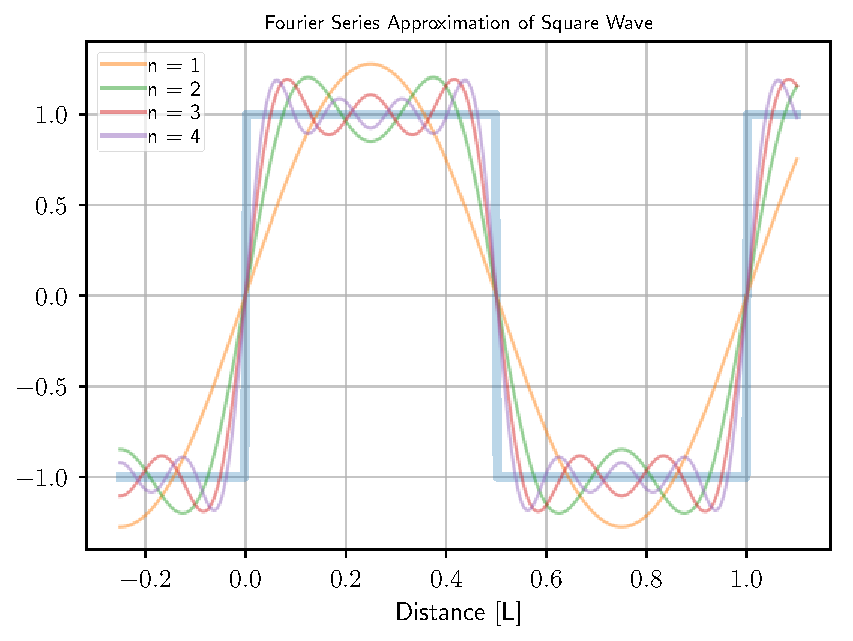
\includegraphics[width=0.5\textwidth]{../../Simulations/FourierSquareWave.pdf}

\end{frame}



\subsection{Compute the Fourier Coefficients}
\begin{frame}
\frametitle{Analogy with Vectors}
\begin{itemize}
\item How to find $B_n$ in $y(x, 0) = \sum_{n=1}^{\infty} B_n
  sin(\frac{n \pi x}{L})$ ?
  \pause
\item When we have a 3D vector ($\vec{z} = a_1 \vec{x_1} + a_2 \vec{x_2} +
  a_3 \vec{x_3}$), we know that we can find the coefficients by using
  the \emph{dot product}: $a_i = \vec{z} \cdot \vec{x_i}$.
  \pause
\item This gives the correct
  answer because the Cartesian basis vectors are \emph{orthonormal}:
  \pause
\item \begin{equation}
        \vec{x_i} \cdot \vec{x_j} = \begin{cases}
          1, & i = j \\
          0, & i \ne j
          \end{cases}
      \label{eq:orthovec}
      \end{equation}
      \pause
\item This works in this straightforward way for any number of spatial dimensions.

\end{itemize}

\end{frame}




\begin{frame}
\frametitle{Orthogonality of Sine waves}
\begin{itemize}
\item This works in the same way for sine, cosine, and complex
  exponentials.
  \pause
\item \begin{equation}
    \frac{2}{L} \int_{0}^{L} sin(n \frac{\pi x}{L}) sin(m \frac{\pi x}{L}) dx
    = \begin{cases}
      0, & m \ne n \\
      1, & m = n
      \end{cases}
      \label{eq:orthosines}
    \end{equation}
    \pause
\item Eq.~\ref{eq:orthosines} exploits the same orthogonality property as
  Eq.~\ref{eq:orthovec}, but over the frequency domain instead of
  space. We can, therefore, use the same technique to get the coefficients.
  \pause
\item Instead of the 'dot product', we'll use the \emph{inner
    product} which is a more generalized kind of dot product.

\end{itemize}
\end{frame}


\begin{frame}
\frametitle{Integrate to find the Fourier Coefficients}
  \pause
We would like to find coefficients $B_n$ and $C_n$:
\begin{align}
  y(x, 0) &= \sum_{n=1}^{\infty} B_n sin(\frac{n \pi x}{L}) \\
  \dot{y}(x, 0) &= \sum_{n=1}^{\infty} \omega_n C_n sin(\frac{n \pi x}{L})
\end{align}
  \pause
Integrating the functions $y$ and $\dot{y}$ with each of the sine waves:
  \pause
\begin{align}
B_n &= \frac{2}{L} \int_{0}^{L} y(x,0) sin(n \frac{\pi x}{L}) dx \\
C_n &= \frac{2}{L} \int_{0}^{L} \dot{y}(x,0) sin(n \frac{\pi x}{L}) dx
\end{align}
\pause
this recipe can now be applied to find the Fourier frequencies of any\footnotemark
function on the domain that respects the boundary conditions.


\footnotetext[1]{See, however, the \href{http://mathworld.wolfram.com/GibbsPhenomenon.html}{Gibb's Phenomenon}}
\end{frame}


\begin{frame}
\frametitle{Example: The Square Wave}
The Square Wave:
\begin{equation}
y(x,0) = \begin{cases}
+1, 0 < x < L/2 \\
-1, L/2 < x < L
\end{cases}
\end{equation}
plot square wave

Integrating the functions $y$ and $\dot{y}$ with each of the sine waves:
  \pause
\begin{align}
B_n &= \frac{2}{L} \int_{0}^{L} y(x,0) sin(n \frac{\pi x}{L}) dx \\
C_n &= \frac{2}{L} \int_{0}^{L} \dot{y}(x,0) sin(n \frac{\pi x}{L}) dx
\end{align}
table of coefficients...
\end{frame}

\begin{frame}
\frametitle{Decomposed Square Wave}

\centering
\includegraphics[width=0.9\textwidth]{../../Simulations/FourierSquareWave50.pdf}


\end{frame}

\begin{frame}
\frametitle{Decomposed Square Wave}
\begin{columns}
\begin{column}{0.5\textwidth}
  \centering
  \includegraphics[width=1\textwidth]{../../Simulations/FourierSquareWave50.pdf}
\end{column}
\begin{column}{0.5\textwidth}
  \centering
  \includegraphics[width=1\textwidth]{../../Simulations/FourierSquareWavePSD.pdf}
\end{column}
\end{columns}

\url{https://github.com/rxa254/VibrationsAndWaves}

\end{frame}


\section{Normal Modes}
\begin{frame}
\frametitle{Normal Modes of a String}
\begin{columns}

  \begin{column}{0.4\textwidth}
    \centering
    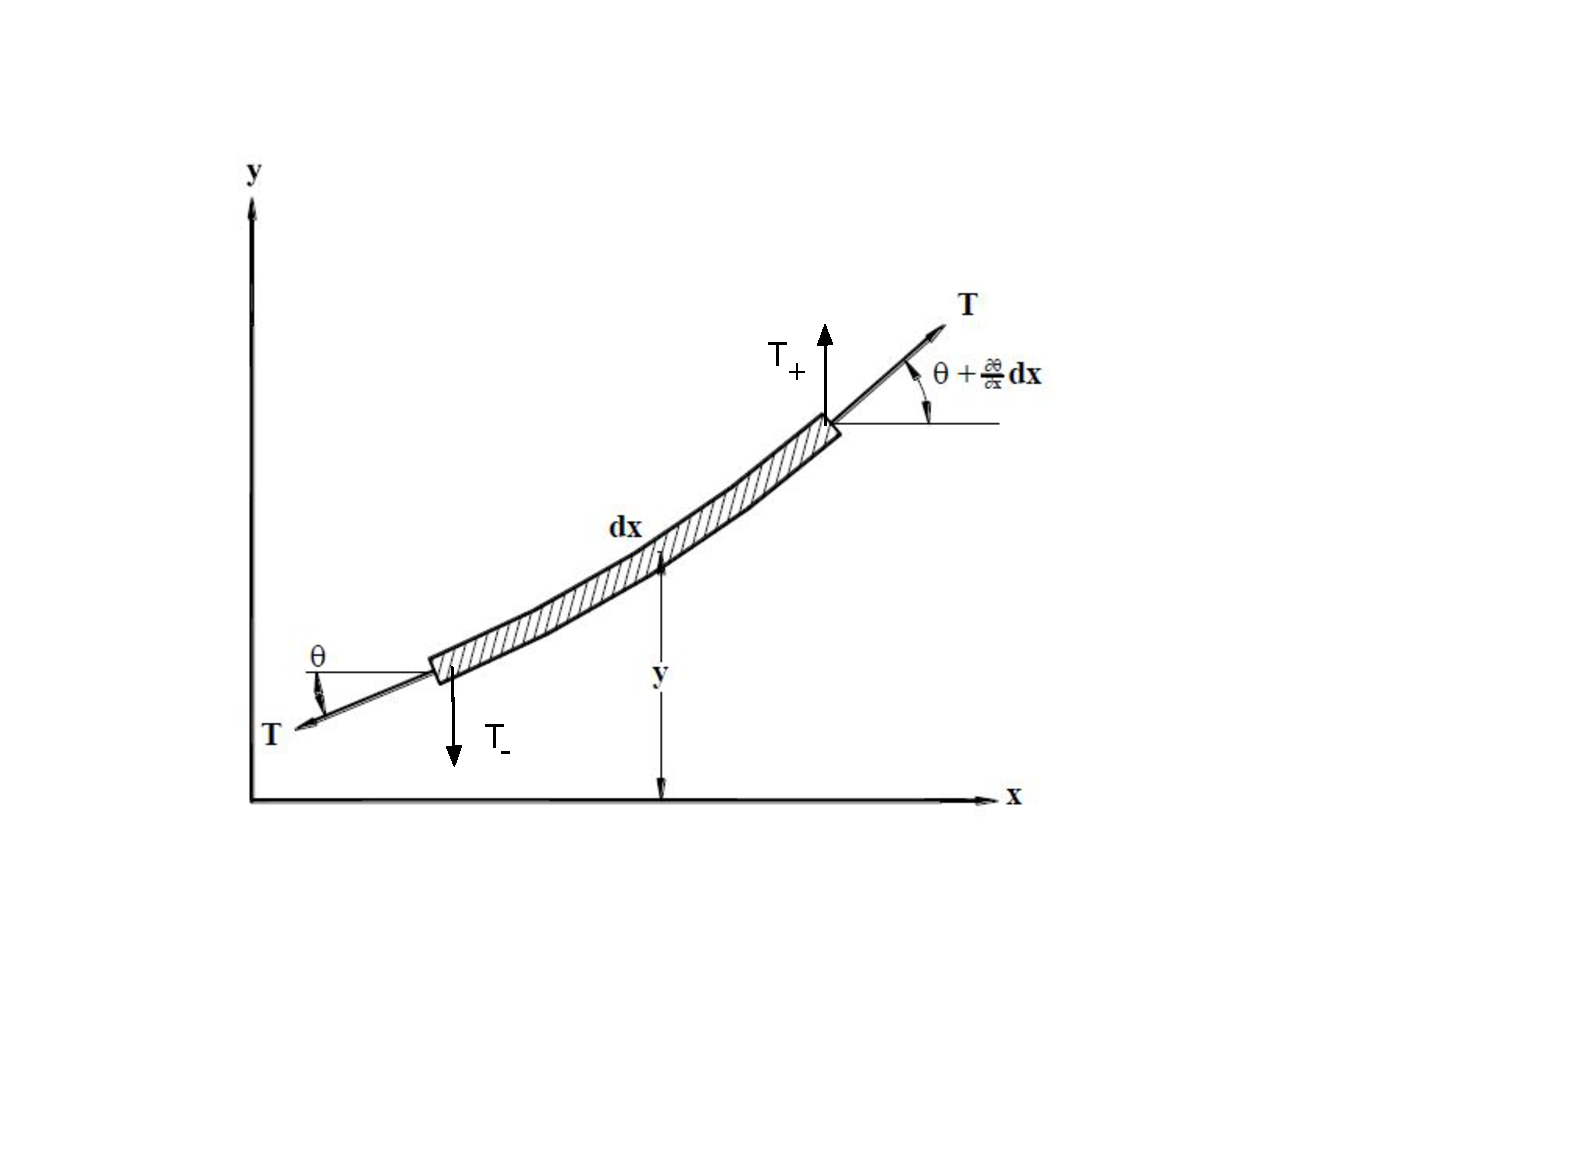
\includegraphics[width=0.85\textwidth]{StringForceDiagram.pdf}

  \end{column}

  \begin{column}{0.6\textwidth}
\begin{block}{The Wave Equation}
\centering
$ \frac{\partial^2 y}{\partial t^2} = \frac{T}{\mu} \frac{\partial^2 y}{\partial x^2}$
\end{block}
\pause
\begin{alignat}{2}
\frac{d^2 g}{dt^2} &= \omega^2 g  &\quad g(t) &= C_1 cos(\omega t) \\
\frac{d^2 f}{dx^2} &= -k^2 f &\quad f(x) &= A cos(k x) + B
sin(k x) 
\end{alignat}
\pause
where the velocity of the wave, $v \equiv \sqrt{\frac{T}{\mu}}$,
$\frac{\omega}{2 \pi}$ is the frequency, and $k \equiv \omega / v$ is
called the 'wave number'. For the wavelength of the wave, we use the
symbol $\lambda \equiv \frac{2 \pi}{k}$.

  \end{column}

\end{columns}

\end{frame}

\begin{frame}
\frametitle{Normal Modes of a String}
\begin{columns}

  \begin{column}{0.4\textwidth}
    \centering
    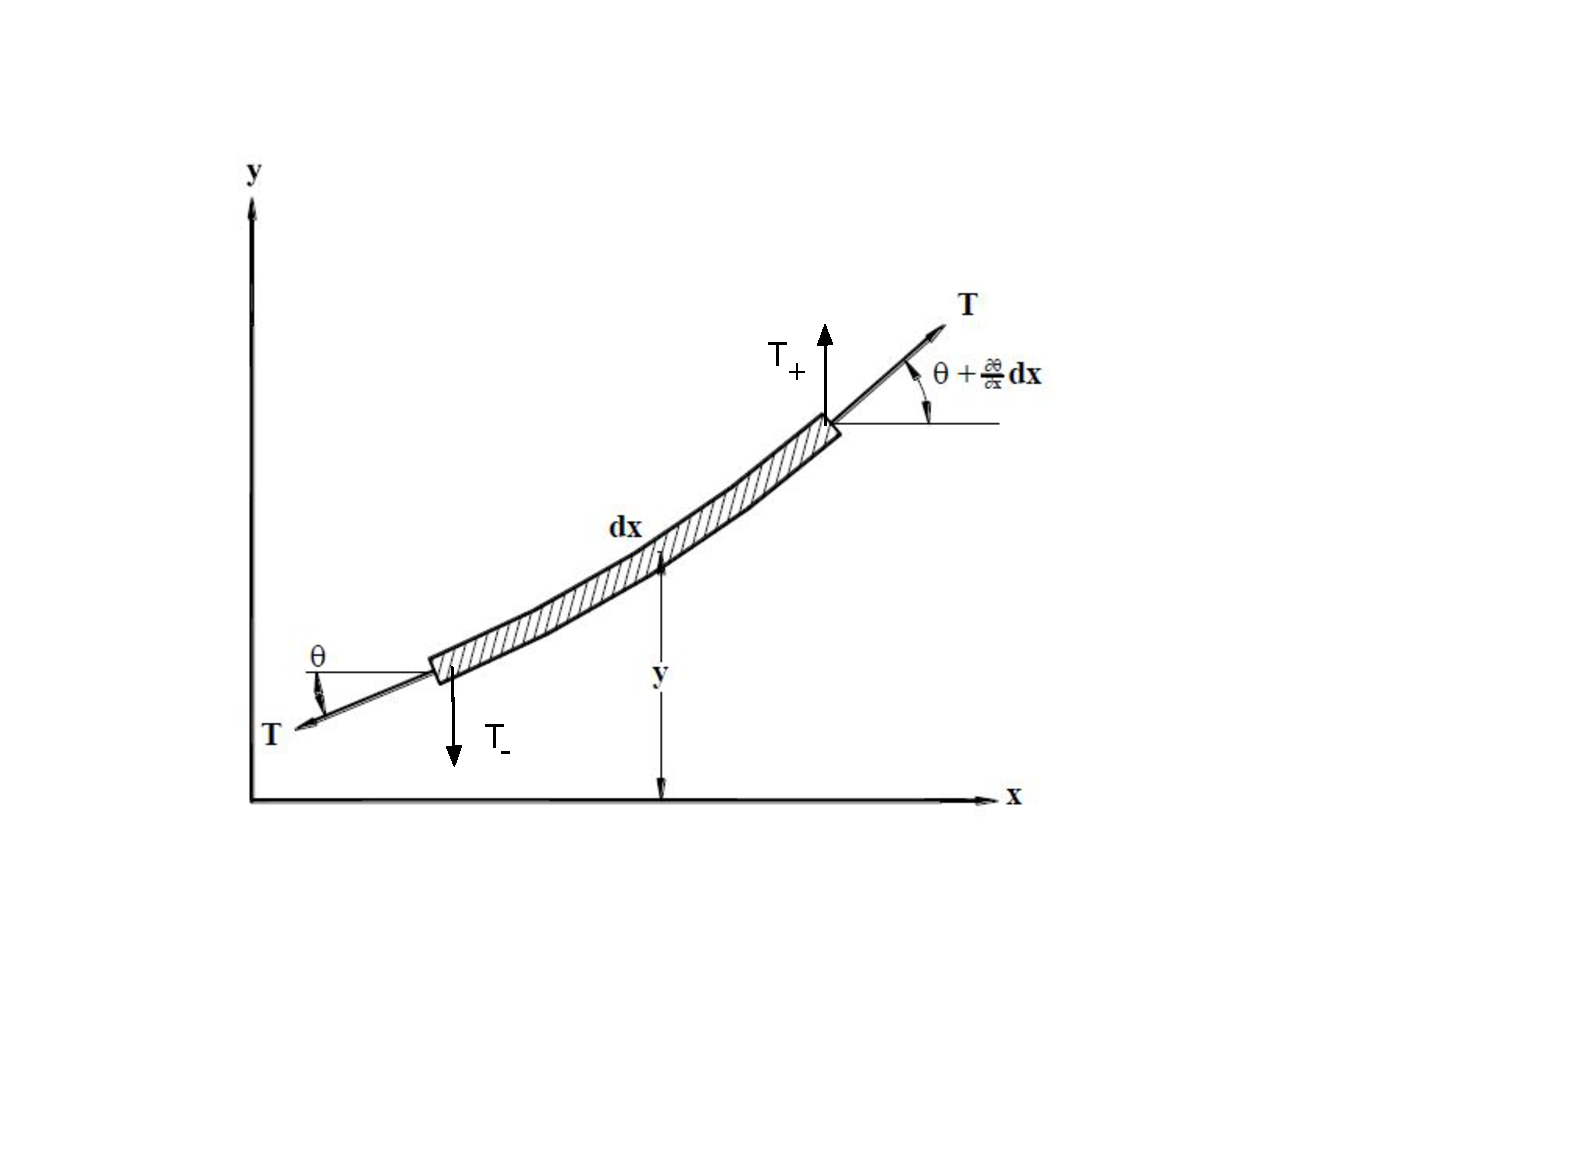
\includegraphics[width=0.85\textwidth]{StringForceDiagram.pdf}

  \end{column}

  \begin{column}{0.6\textwidth}
    \begin{enumerate}
    \item $f(x) = 0$ for $x \in \{0, L\} \implies$ \\
      \pause
    \item $sin(k L) = 0$ for any and all t, and $A = 0$\\
      \pause
    \item so $k_n L = n \pi$ or $k_n = n \frac{\pi}{L}$ \\
      \pause
    \item and $y(x, t) = A_n cos(\omega_n t) sin(k_n x)$ \\
    \end{enumerate}

  \end{column}

\end{columns}
\pause
In this case, the boundary conditions preclude cosine terms, but
for strings without fixed ends we would include both sine and cosine.

\end{frame}

\section{Summary}
\begin{frame}
\frametitle{Summary}
\pause
\begin{itemize}
\item Fourier Analysis: decompose solutions into sinusoidal components
  of different frequencies
  (French pp. 189\,--\,196)

\item $y(x, t) \rightarrow \tilde{y}(f, t)$

\item The \emph{Fourier Transform} converts a function from the
  time-domain into the frequency-domain.

\item Functions which are made up primarily of sinusoids are
  efficiently described in the frequency domain (e.g. harmonic
  oscillators) using tools like the Bode Plot and Power Spectrum.

\item We know the SHO solutions are just sinusoids, so \emph{any}
  arbitrary shape, $y(x,t)$, can be decomposed into these Fourier
  components and then evolved in time.

\item The most general solution is an infinite sum over the
  eigenfunctions: \\
  $y(x, t) = \sum_{n=1}^{\infty} A_n cos(\omega_n t) sin(k_n x)$

\end{itemize}


\end{frame}

\end{document}

